\documentclass[final]{cmpreport}

\usepackage{enumitem}
\usepackage{wasysym}
\usepackage{framed}
\usepackage{pgfgantt,rotating}
\usepackage{subfloat}
\usepackage{listings}
\usepackage{xcolor}
\usepackage{colortbl}
\usepackage{url}
\usepackage{hyperref}

\usepackage{color}
  \definecolor{lightgray}{rgb}{0.95, 0.95, 0.95}
  \definecolor{darkgray}{rgb}{0.4, 0.4, 0.4}
  \definecolor{purple}{rgb}{0.65, 0.12, 0.82}
  \definecolor{otherCode}{rgb}{1, 0.5, 0} % #FF7F00 -> rgb(239, 169, 0)
  \definecolor{blueCode}{rgb}{0, 0, 0.93} % #0000EE -> rgb(0, 0, 238)
  \definecolor{greenCode}{rgb}{0, 0.6, 0} % #009900 -> rgb(0, 153, 0) 
\usepackage{upquote}
\usepackage{listings}
\makeatletter
\lstdefinelanguage{HTML5}{
  sensitive=true,
  keywords={%
  % JavaScript
  typeof, new, true, false, catch, function, return, null, catch, switch, var, if, in, while, do, else, case, break,
  % HTML
  html, title, meta, style, head, body, script, canvas,
  % CSS
  border:, transform:, -moz-transform:, transition-duration:, transition-property:,
  transition-timing-function:
  },
  % http://texblog.org/tag/otherkeywords/
  otherkeywords={<, >, \/},   
  ndkeywords={class, export, boolean, throw, implements, import, this},   
  comment=[l]{//},
  % morecomment=[s][keywordstyle]{<}{>},  
  morecomment=[s]{/*}{*/},
  morecomment=[s]{<!}{>},
  morestring=[b]',
  morestring=[b]",    
  alsoletter={-},
  alsodigit={:}
}
\lstset{%
  % Basic design
  backgroundcolor=\color{lightgray},
  basicstyle={\tiny\ttfamily},   
  frame=l,
  % Line numbers
  xleftmargin={0.75cm},
  numbers=left,
  stepnumber=1,
  firstnumber=1,
  numberfirstline=true,
  % Code design
  identifierstyle=\color{black},
  keywordstyle=\color{blue}\bfseries,
  ndkeywordstyle=\color{greenCode}\bfseries,
  stringstyle=\color{otherCode}\ttfamily,
  commentstyle=\color{darkgray}\ttfamily,
  % Code
  language={HTML5},
  tabsize=2,
  showtabs=false,
  showspaces=false,
  showstringspaces=false,
  extendedchars=true,
  breaklines=true
}
\makeatother

\title{Building a Cross-Platform\\Mobile Game with HTML5}

\author{Joshua Barnett}

\registration{5939968}
\supervisor{Professor Andy Day}

\ccode{CMPC3P2Y}

\summary{
Creating cross-compatible games is a necessity for aspiring developers. The more platforms a game supports, the wider an audience the developer can reach, and therefore their potential for success. Nowhere is this more evident than the mobile gaming market. However, the platform fragmentation associated with mobile devices impedes the development process, as tailoring an application to every device is impractical, and in most cases extraneous. One attractive solution to this impediment is targeting the web platform that constitutes openness and inherent portability.

This project aims to explore the web platform's pros and cons by researching technologies on offer to developers. These technologies will then be assessed through the creation of a mobile game by rating the ease of development and deployment when compared to conventional native development. 

Full assessment of the field would require an analysis of both native and non-native development. However, the scope of this project does not allow me to do both. Therefore, the focus of this project will revolve around HTML5 and the web platform. While HTML5 will constitute the focus of my analysis – this is what I have used to build my prototype mobile game – I will refer to native development from my personal observations and apparent evidences as a means to provide field for comparison and give depth this project. I feel this project will encourage me to research and learn these emerging technologies, and the knowledge gained will provide me with a strong footing for my desired career in industry.
}

\acknowledgements{
I would like to thank Professor Andy Day for supporting this project with and its fluctuating nature. My parents Paul and Jane for cultivating and enabling my technical and creative characteristics. As well as Elise Lanteri for her superior grasp of english grammar and the written word.
}

\begin{document}

\section{Introduction}

During the past five years the popularity of mobile devices has been increasing. These devices have become one of the foremost ways in which the modern world consumes media and entertainment. Original equipment manufacturers (OEMs) such as Apple, LG, Nokia, and Samsung, have become progressively competitive in producing better mobile devices for the global market, generating a variety of them in the process. This growing market constitutes a large audience for mobile applications which conscientious developers aspire to target. However, in order for a mobile application to succeed in such a competitive and saturated market, it is a necessity that they support as many devices as possible; the more devices an application supports, the wider an audience it can reach. Now, currently, this is an arduous process, as each mobile device falls into a subset of operating systems and hardware specifications. Each operating system has a different application programming interface (API), which is made accessible through its corresponding software development kit (SDK). Hence, for a developer to target each operating system `natively' the development of the application must vary, and be adapted. This native adaptation process is an inefficient approach to cross-compatible mobile game development. It requires more time, people, and, consequently, money. At the core of this project's research is the exploration of a solution to this deterrent that developers face.

The Open Web Platform (OWP) in essence is a collection of open (royalty-free) technologies that can be used for application development. The standards for these technologies defined by the World Wide Web Consortium (W3C) to standardise and maximize a consensus amongst its members. Web applications built with these technologies benefit from the inherent portability of the Web, meaning they can be universally executed and distributed amongst a wide range of devices. Modern mobile devices fall into a subset of this range, as they contain essential software such as web browsers that can render and run web pages used to deliver the OWP. This makes the OWP an appealing free alternative to that of developing natively for each mobile operating systems, as the requirements for cross-compatibility are minimized.

HyperText Markup Language (HTML) is the corner stone technology of the OWP. Its purpose is to specify the content of a web page. The fifth iteration of HTML (HTML5) has further broadened the types of content that it can deliver. Now, allowing for the definition of rich interactive content such as audio, video, and a graphics within the page. HTML5 and its associated technologies can be leveraged by developers to create mobile games that support the variety mobile devices. This project will focus on the usage of HTML5 and its companion technologies in mobile game development. In order to do so I have decided to build a game using HTML5 so that I could, along the way, assess the ease of development and deployment, as well as the difficulties arising from it.

\section{Background}

``HTML5'' is a confusing term because it has been associated with many aspects of modern web development. At its centre it is the fifth iteration of the HTML language specification, but, it is also a umbrella term that encompasses all of its companion technologies.

Hybrid application frameworks currently serve developers by providing access to specific device APIs that are either inaccessible or have not yet been implemented to a satisfactory standard. However, as browsers and web views on mobile devices improve and shape web standards these will most likely serve as a stop gap until better support for HTML5 applications exists. When transitioning from a hybrid application to solely HTML5 the underlying source code will still be compatible, and if engineered sensibly it will also require minimal changes.

has become an all encompassing term that includes a host of technologies, because alone this language cannot fully deliver rich web experiences. Technologies such as JavaScript (JS), Cascading Style Sheets (CSS), Scalable Vector Graphics (SVG), the Document Object Model (DOM) and WebGL have also been playing an integral part in shaping the modern web landscape. When used together in various combinations, these form a Web Platform\footnotemark on which to convey content and information in new and interesting ways. It is currently the convention to refer to this new platform as solely HTML5 because this is where all these technologies stem from.
\footnotetext{\url{http://docs.webplatform.org/wiki/Main_Page}}

``Linux'' has similarly been distorted as an umbrella term for Linux based operating systems such as Debian, Fedora, and Ubuntu. Nevertheless, ``Linux'' alone is just the open-source kernel which lies at the heart of these distributions which on its own would not be of much use.

\section{Design}

\section{Implementation}

\section{Conclusion}
HTML5 is the fifth iteration of the hypertext mark up language. During its previous iterations such as HTML 4.01 and XHTML 1.1 there was minimal support for multimedia content. This resulted in a void that was promptly filled by third-party plugins such as Adobe Flash and Microsoft Silverlight. Such plugins allowed for easy presentation of media such as video, audio and even allowed for interactivity that was used to great effect in games.

Unfortunately many of these plugins are proprietary and closed-source which prevents developers from fixing and debugging inherent issues in the technology. Instead they are dependant on the technology owner for solutions while being limited to reporting them or finding ``temporary'' workarounds. Plugins often require some form of installation process as they are ``add-ons'' and exist outside of scope of the W3C standards.

\citet{Jobs} famously professed his concerns about Flash and presented sound reasoning as to why Apple had no intentions of supporting or integrating Flash into their iOS devices. Flash was also briefly available for Android but was short lived and eventually discontinued by Adobe. Adobe is continuing to making strides into the mobile platform with their new runtime AIR\footnotemark. HTML5 is still currently a work in progress but the \cite{W3C} have made plans to stabilize the specification and help it reach \textit{Recommendation\footnotemark} status as of this year.

\footnotetext{\url{https://www.adobe.com/aboutadobe/pressroom/pressreleases/201002/021510FlashPlayerMWC.html}}
\footnotetext{\url{http://www.w3.org/2005/10/Process-20051014/tr.html\#rec-publication}}

The DOM is the core of what drives modern web applications. It provides a means to manipulate the structure and style of the original document loaded from a web server at run-time on the client side.

What makes HTML different from most compiled languages such as C++ and Java, is its a interpreted language. Compiled languages are typically converted into a binary format that compresses their instructions into machine-code allowing for quicker execution. Interpreted languages such as Python and Ruby in contrast are often read line-by-line with their instructions parsed and executed at run-time.

When HTML is interpreted by a web browsers it is parsed into a DOM. The DOM is essentially a representation in memory of what was originally marked down in the static HTML document. This allows the browsers to interpret relations between elements and use them to render the document appropriately. While in memory the information is not longer static allowing for manipulation by other technologies such as JS.

One example of where this manipulation is used to great effect is the SPA (single-page application). SPAs have significant advantages over that of traditional websites as they can provide a seamless user experience similar to that of desktop applications. Instead of navigating through links that loading separate HTML pages they use states to manage the flow, loading information dynamically when required or requested. This technique shrinks factors such as load times, enables rich interactions, and responsiveness while encouraging reuse. \citep{Takada}

Web browsers are client side applications that render the information requested by the user and then sent from a web server. Many of the popular browser vendors such as Google (Chrome), Apple (Safari), and Mozilla (Firefox) all have a mobile counterpart. However these mobile counterparts often support a subset of features in their desktop editions making much of the fringe HTML5 features even less accessible.

Getting a single web application to render and function consistently across a range of browsers can be a huge undertaking. This task has grown exponentially with the introduction of mobile devices and their endless combinations of hardware, operating systems, and mobile browser applications. Each combination of these variables has the potential to produce unique bugs and quirks specific to a particular test case. As the specification of HTML5 was being developed much of the new features have been implemented in browsers at the discretion of the vendor. This has quickly led to cross compatibility issues as older browsers will support less of these new features and not necessarily be consistent with the other browsers that were available at the time.

Depending on the project specification a developer can rapidly become limited by what features of HTML5 they can utilise. For instance one such feature that was initially being used to develop \textit{MindFlip} was \textit{viewport units}. This feature allows for the scaling of elements based upon the current viewport's dimensions which is especially useful on mobile devices for scaling visual elements relative to the screen's aspect ratio and pixel density. However the stock web browsers on mobile devices have only recently added support for this feature with it being introduced in version 4.4 of Android and 6.0 of iOS.

\begin{figure}[h]{A compatibility table for viewport units \label{viewport}}
  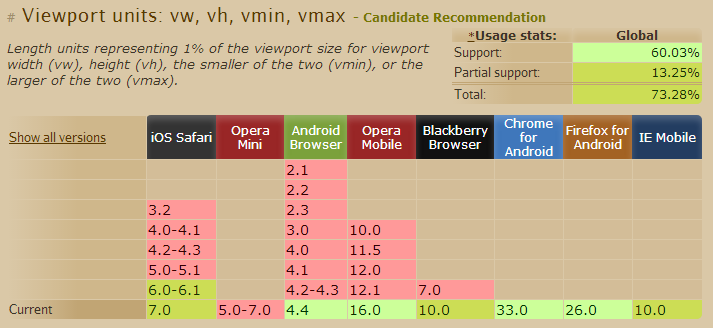
\includegraphics[width=1.0\textwidth]{viewport-units.png}
\end{figure}

In cases like these a developer can either limit their platform target range and make use of the fringe features or use a polyfill also known as a shim. A polyfill is often referred to as code that substitutes the lack of a future API (application programming interface) by utilising existing features to mimic that of newer fully fledged implementations \cite{Lawson}. In the case of this project the lack of \textit{viewport units} support in older mobile browsers present an issue. After searching for a solution the presentation slides of \cite{Kadrmas} detailed a technique using \textit{em} units in HTML5 mobile games. \textit{em} units were originally intended for scaling DOM elements relative to the current font size. This technique was implemented in the project and allowed the game to correctly scale across differing screen sizes. When a window \texttt{resize} event is dispatched the \texttt{resize} function in \texttt{viewport-model.js} uses the window's current dimensions to set its values appropriately. These changes in the model are then listened for by \texttt{viewport-view.js} then applies them to the \texttt{viewport <div>} element. By changing the font size of the root (viewport) element relative to the window's width, all the contained elements also inherent this \texttt{font-size} CSS property which can then be used through the use of \textit{em} to scale individual elements. This approach also made it easy to retain a specified aspect ratio, preventing any oddities when displaying on landscape displays.

\clearpage
\begin{lstlisting}
resize: function (e) {

    var xwindow = window.innerWidth;
    var ywindow = window.innerHeight;

	// e.g. 16:9 or 4:3 screens.
    var xratio = this.get('xratio');
    var yratio = this.get('yratio');

    var landscape = window.innerWidth / xratio;
    var portrait = window.innerHeight / yratio;

    if (landscape < portrait) {

        this.set('width', Math.round(xwindow));
        this.set('height', Math.round(xwindow * (yratio / xratio)));

    } else {

        this.set('width', Math.round(ywindow * (xratio / yratio)));
        this.set('height', Math.round(ywindow));

    }

	// used by 'viewport-view.js' to set css('font-size').
    this.set('scale', Math.floor(this.get('width') / 3));

}
\end{lstlisting}

However, even when polyfilling potential feature gaps in browsers, issues can still occur under a variety of circumstances. One of the most reliable ways to ensure compatibility is to actually test on all the mobile devices in the target range. This solution most of the time is impractical, especially funds are limited. The next best alternative is to either emulator such devices or use online tools such as BrowserStack\footnotemark. Figure \ref{browserstack} shows thumbnails of \textit{MindFlip} on Android and iOS browsers this is a helpful utility that assists in highlighting obvious incompatibility issues at a glance. The blank thumbnails quickly point out where my game is not loading, which allows for selection and prioritizing of what devices need in depth debugging. However, limited workforce, budget, and time meant this project could really only afford to comprehensively debug devices at hand such as the Samsung Galaxy S4 and the Google Nexus 7 (2012).

\footnotetext{\url{http://www.browserstack.com/}}

\begin{figure}[h]{Screenshots of MindFlip on various mobile device browsers \label{browserstack}}
  \centering
    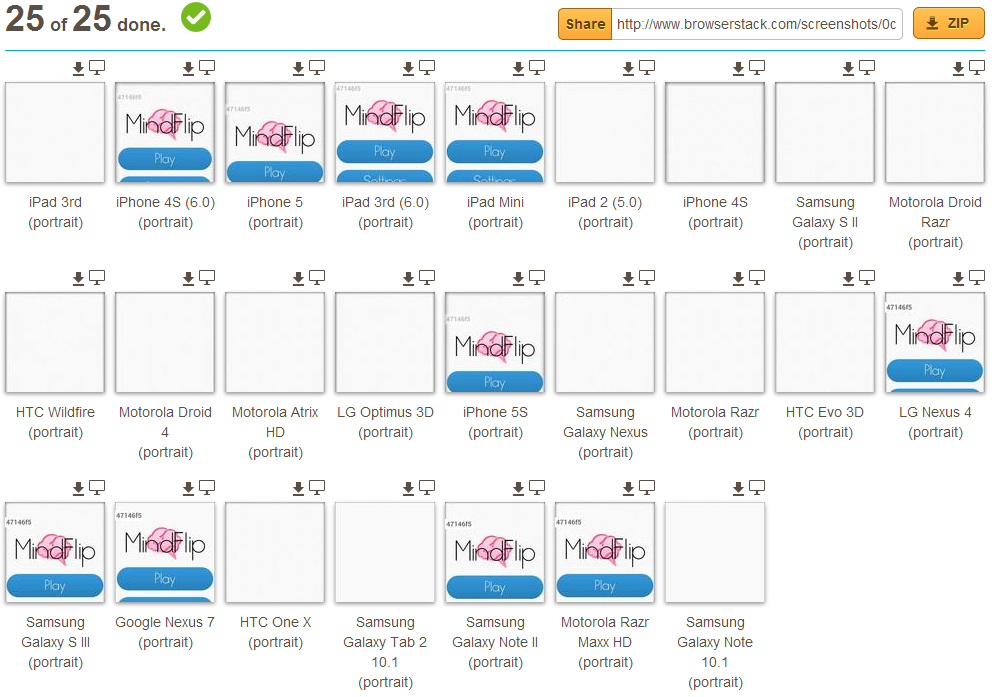
\includegraphics[width=0.8\textwidth]{browserstack.png}
\end{figure}

\clearpage
Rendering graphics for video games through HTML5 is possible through a variety of ways. DOM based games use elements and styles effectively and take advantage of the browser's long standing rendering conventions. However, most game developers are more familiar with rendering through the rasterization of a graphics layer which can be manipulated at runtime. Both of these approaches are now possible on mobile devices as of recent developments but there is still room for improvement.

The fundamentals of web development are that the content of a website is typically marked down in a \texttt{.html} document and the style of this content is embedded alongside or defined within a \texttt{.css}. The browser parses the rules found in the stylesheet identifying referenced document elements in the process. This information then instructs the browser how to render the selected document elements often improving their otherwise bland presentation. Although HTML has been getting a much needed update, this begs the question of what its companion CSS has been doing in order to enhance the web experience. 

The latest iteration of CSS often referred to as CSS3 provides new and interesting ways in which to style these elements. Notable features include rounded corners, shadows, gradients , transitions or animations , as well as new layouts like multi-columns , flexible box or grid layouts\footnotemark.

\footnotetext{\url{https://developer.mozilla.org/en-US/docs/Web/CSS/CSS3}}

The support for these on mobile browsers has been around for quite awhile with much of the older versions supporting them through the use of vendor prefixes. These are a side effect of specification CSS3 still being a draft as such features were classified as experimental at the time. However, these are starting to be phased out as browser vendors start to agree on specifics and it also provides a means in which to use them providing legacy support for older browsers.

Canvas is probably the most significant feature that was introduced in HTML5, especially for game developers. It finally enables developers to do interactive and dynamic graphics natively in the browser, without third-party plugins.

The new \texttt{<canvas>} element defines a graphics layer in a HTML document that can be manipulated and drawn to through a JavaScript API. Although this has been used in the context of desktop web applications to great effect it has suffered from performance issues on mobile browsers. This is often due to being limited to software rendering that only makes use of the device's CPU. However, the performance of mobile devices has been increasing recent years with an emphasis on GPU development \cite{Lin}. This has led to browser vendors adding support for GPU accelerated rendering on mobile devices in places that use complex effects such as CSS3.

However utilisation of these faster processors with the canvas element has only just started to become common place. There are many ongoing software projects with a focus on accelerating the HTML5 canvas using the mobile device's GPU. Unfortunately there is a lack of cross platform open-source projects that tackle this issue. Ejecta is an is one such project but it current only supports iOS and the hybrid mobile application framework Apache Cordova\footnotemark also provides an accelerated canvas through a plugin called FastCanvas\footnotemark.

\footnotetext{\url{https://cordova.apache.org/}}
\footnotetext{\url{http://plugreg.com/plugin/phonegap/phonegap-plugin-fast-canvas}}

WebGL is a distillation of the popular OpenGL making GPU accelerated rendering in the browser now a reality. WebGL, a JavaScript API is based on the OpenGL ES (Embedded Systems) subset, and as the name implies it was designed and optimized for embedded systems such as mobile devices. One streamlined modification OpenGL ES made was the removal of the fixed-function API introduced in OpenGL 1.0 enabling the use and compilation of modern shaders.

WebGL has been in development for the past three years which came to maturity as of early last year when the first a stable version was released. As this is a new technology it has only just begun surfacing in the wild, one notable example is the PlayStation 4's user interface. In a revealing presentation given by \cite{Olmstead} it was declared that the move to WebGL was done to ensure cross platform support. This potentially hints at Sony's future plans to bring their games to multiple platforms including mobile devices through their PlayStation Now streaming service.

However, the support for WebGL through mobile browsers is essentially nonexistent to date. One company striving to change that is Ludei, who are in the early stages of rolling out their new technology CocoonJS. CocoonJS is a means of packaging and publishing HTML5 applications on mobile devices. In amongst this framework is the facilitation of WebGL letting it tap into the onboard GPU available on most modern mobile devices. Many of the demos they provide demonstrate close to near native performance. This makes WebGL a feasible avenue for game development on mobile devices, with the added bonus of being cross platform ready.

The state of HTML5 audio support in mobile browsers at this present time is still very limited and plagued with issues. Audio is a key component in delivering a satisfying game experience as it provides stimuli and feedback to the player. This can help further immerse the player in the game experience especially in main stream AAA games. However, audio can play a part in mobile games too emphasising and cuing player interaction that would otherwise be difficult to prompt without the use of popups and explanatory text. These latter techniques are often avoided because they can bore and frustrate the player while breaking their immersion in the process. Audio can also serve as a brand mechanism for mobile games providing a strong theme that could be associated with good quality experiences.

Commonly the first action most players will take when playing a mobile games to instant mute or lower the audio. Players have a very low tolerance for disturbing sound design and due to earlier mobile games have been conditioned in this way. This stresses that audio must be used sparingly and in the appropriate context in order to deliver the full intended game experience \cite{Thomas}.

The \texttt{<audio>} element is another significant addition from the HTML5 specification. It provides developers a way to define sound content within a HTML document which can then be loaded and played back by web browser. Because of this element web applications can now finally deliver an audio experience that before was impossible to achieve without the use of a third-party plugin.

Support for this element in mobile browsers is widespread however there are many discrepancies between them. Here is a list of some of the known issues that currently effect mobile browsers taken from \textit{caniuse.com\footnotemark}.

\footnotetext[8]{\url{http://caniuse.com/\#feat=audio}}

\begin{itemize}
  \item Audio played from the element in iOS always plays in a full screen player.
  \item Playback rate not supported on the stock android browser.
  \item Only one Audio file can be played at one time in iOS and Android browsers which forces you to use sprites for multiple audios.
  \item Audio in iOS can not be auto played. It even starts downloading after a user triggered event.
  \item Volume is read-only on iOS.
\end{itemize}

Much of these restrictions imposed by mobile web browsers make it awkward to utilise \texttt{<audio>} as an competent solution for dynamic sound effects and background music. This also poses a problem when trying to compete with native mobile games as features such as multichannel audio and equalizers come standard with their relative SDK.

The Web Audio API is an experimental high-level JavaScript API that is currently being drafted and developed by Google and the W3C\footnotemark. This API provides richer methods to manipulate and generate audio through signal processing and synthesis. This also includes the ability to load and playback audio files similar to the \texttt{<audio>} element. A similarly the MediaStream API\footnotemark developed by Mozilla is trying to achieve the same functionality focusing on the streaming of both audio and video related data.

\footnotetext{\url{http://www.w3.org/TR/webaudio/}}
\footnotetext{\url{https://developer.mozilla.org/en-US/docs/WebRTC/MediaStream_API}}

This definitely appears to be a more appropriate technology for the implementation of game related audio. However, these technologies are much newer than the \texttt{<audio>} element and have yet to be implemented in any of the stock mobile browsers with the exception of iOS Safari versions \texttt{6.0-7.0\footnotemark}.

\footnotetext{\url{http://caniuse.com/\#feat=audio-api}}

With the advent of hybrid mobile applications frameworks in some cases it is now viable to bridge to the mobile operating system's native media player. This presents much fewer headaches to developers as these APIs have been around for much longer and are therefore adequately stable.

The game utilises Apache Cordova which has an official plugin that bridges the gap from JavaScript to most naive mobile media players. This allowed me to make calls to the Media plugin's API and have the native media player load and playback audio files that were in my web applications directory. Unfortunately Cordova's official Media plugin had quite high latency which detracted from the tactile feel that improves the user's experience. Research yielded a custom LowLatencyAudio plugin that had been developed by \citep{Trice} for the PhoneGap framework (the predecessor to Cordova). This plugin was since ported to Cordova by \citep{Xie} for Android and iOS which was used to solve the tactility issue.

When designing any game it is pertinent that the player enjoys their participation in the game experience. Enjoyment can take many forms, but the majority will boil down to the player obtaining satisfaction from learning. Typically when successfully emulating a mental model akin to that of the game's underlying flow and structure. This allows for the prediction of cause and effect that takes place within the game's system, \cite{Cook}. Yet when the terms of engagement with the game change drastically from the norm such as the means of interaction, such is the case with mobile games. It creates an added layer of design complexity that is required for the system to provide sufficient accessibility and feedback to the player.

The choice of interface should be highly weighted relative to the context of the game system. For instance a real-time game system would not be suited to that of a touch interface that simulates a conventional input system such as buttons (unless highly simplified). This is because it lacks tactile feedback and indirectly effects gameplay, creating a sense of incoherence in the user experience. This method however could be applicable in the context of non-gameplay sections such as menu navigation and non real-time game systems such as turn-based game genres, \cite{XuBradburn}. In these systems because there is no emphasis on player reaction time it lends itself to such interface methods. One advantage to this approach is the omission of a tutorial as most players are accustomed to such conventions.

A better route still is to provide an intuitive means of interface with the game system that could enhance the game experience. Good examples of touch interfaces often take a minimal approach, consisting of few touch gestures, this has substantial benefits over that of the simulated. Angry Birds\footnote{\url{http://www.angrybirds.com/}} is a classic example of an intuitive touch interface because the gestures made by the player have direct correlation to visual feedback on the screen. Once the gesture is made the game system simply uses your interaction as the seed of entropy that is then played out (using a physics engine). All the while allowing the user to clearly observe the cause and effect in the game system. Their interaction only formed the initial section of the game loop and for the rest was not obscuring the visual feedback.

User-centred design (UCD) is an interesting approach to mobile game design, instead of relying solely upon the experience and vision of designers it considers the potential future players of the game to be the core design informant. At the core of any game design process is objective to create a meaningful game experience for the player. Two key factors in achieving this are discernibility; providing the player feedback on their actions, and integration; showing the player their actions and outcome in the larger context of the game system.

One positive effect of this perspective on game design is it avoids the potential pitfalls that stem from designers. Designers can have a tendency to ``fall in love'' with their own game ideas as it often originates from their own desires as to what they look for in a game experience. Such approaches may misrepresent what the user base wants from their game experience, as it suffers from lack of wide initial feedback and criticism. The design process is a means to combine logic and information to form satisfactory choices to base a game's blueprint on. The information on which the logic is built can be yielded from a variety of sources; research literature, statistical data, player feedback and the designer's own input, \cite{ErmiMayra}.

Dependant on what root is taken when developing an application for the mobile platform most software engineering strategies can be applied through some form. A popular strategy is unified modelling language (UML) which can be applied in the context of mobile game development, \cite{UML}. However the advantages presented in this method of this approach may be better suited to that of a business software context. It has the potential hinder development of an evolving interactive application by restricting the ability to create through quick iterative prototyping. Especially in the context of a small development team with a limited development time frame.

``Game mechanics are rule based systems or simulations that facilitate and encourage a user to explore and learn the properties of their possibility space through the use of feedback mechanisms.''\cite{Koster} Games are engineered to provide enjoyment and a sense of satisfaction for the user. They do this through recording a player's performed action, which in turn causes an effect in the game space. The player then receives feedback often in the form of rewards or new tools which can then be used in the same or newly introduced game mechanics. Human behaviour has made this a good model because we have evolved and survived due to our increasing learning capabilities. The brain's reward centre will release chemicals (dopamine) that encourage such actions during the learning process.

\cite{Skinner} proved with his operant conditioning chamber that not only is it possible to condition human reactions but it is also possible to condition human volition and change the way users make choices. Many successful games that exist in today's market are built on this principle and can sometime exploit its power over their audience. Operant conditioning experiments have shown that to get a player to engage in an activity there must be some sort of feedback that the player takes pleasure in such as a reward. However it has also shown that the best way to get the player to repeat the activity is not to provide feedback consistently. Instead having the feedback be delivered at random intervals or at set time periods has shown to be far more effective.

Games such as World of Warcraft\footnote{http://eu.battle.net/wow/en/} (WoW) and various social games have manipulated this human characteristic beyond their initial novelty. An example of that would be when a player has reached the ``end-game'' (reaching the maximum character level) in WoW , the key activities that are left to engage in are ``raids''. These are large-scale game scenarios that require several participants to progress through various virtual dungeons. Most of these dungeons have character class specific rewards that are delivered upon the defeat of a boss. These rewards however, have a randomised probability of occurring which bares significant similarities with that of the operant conditioning experiments. This game design methodology is not exclusive to that of large scale experiences it can also be applied in a very simplistic context. Examples such as Solitaire\footnote{http://en.wikipedia.org/wiki/Solitaire} and Candy Crush Saga\footnote{http://about.king.com/games/candy-crush-saga} have infrequent reward systems for the player which condition them in a similar way. Nevertheless such experiences may be engaging for the player but this does not make them compelling forms of play, \cite{ExtraCredits}.

The core concept of the game had to be simplistic with room for expansion and modification. This led to the decision of basing it upon simple card game of \textit{Concentration\footnotemark}. The game's core mechanics would consist of the player initially being presented with a set of cards each labelled with a symbol relating to a set. These symbols will only be briefly visible to the player at the start of the game before they are then turned over to obscuring their front-face. This then makes each card indistinguishable from the rest. The player's objective was then to identify matching cards from memory within limitations. This core concept was chosen consciously for a few reasons.

\footnotetext{\url{http://en.wikipedia.org/wiki/Concentration\_(game)}}

\begin{enumerate}
  \item It is relatively simple, making it quick and easy for players of all ages to recognise and understand the core gameplay mechanics.
  \item It has depth, allowing for additional and more complex gameplay mechanics to be introduced gradually to the player.
  \item It will translate well to touch screens, because the fundamental interaction the player will have is selecting cards (whether it be individually or concurrently).
\end{enumerate}

Other mechanics such as matching sets of cards in a specified order were later introduced to put a unique spin on the gameplay. This means players will effectively have to chunk their memories of card positions in particular orders so they can be retrieved later in the reveal stage of the game. Additional shapes and symbols in various placement symmetrical and asymmetrical patterns were also added making players improve their memory capacity and pattern recognition skills.

Throughout the development and prototyping of MindFlip it was important to take into consideration the reactions and feedback of players. So whenever the chance arose I would hand over my phone containing my latest stable build of the game and observe others playing it from a third-party perspective.

Preconceptions can be a double edged sword when used in game design. Often they can be used to draw parallels between activities in contemporary games such as my own. This acts as a shortcut when teaching a player new or similar gameplay mechanics. However, these can also be stumbled upon accidently from a developer's perspective as their own preconceptions about games will likely be vast by comparison to the average player.

This was the case with the initial draft of introductory level. In the beginning the first two card symbols the player encountered were a red nought and a blue cross on a three-by-three grid. After showing the game to my sister while providing no tutorial, the first actions she made were to produce a winning \emph{Tic-tac-toe} game state. This made it apparent that there was a flaw in my game design, because the symbols are common to a pre-existing game namely \emph{Tic-tac-toe} the player receives mixed signals about how to play the game from the offset leading to frustration and confusion. I later decided to go for simpler more abstract symbols such as circles, squares, and triangles in my initial set of levels do to their generic associations they imply simplicity leaving the player open to learn the game mechanics.

When creating a game targeting HTML5 it can be difficult to know what workflow to invest in. Developers each have their own preferences and beliefs as to what is the best way to work with their priorities often being similar but achieved in different ways. It also has useful tools such as watchers which will automatically build and update your preprocessors code

\label{sec:transpilers}

JavaScript in its current state (ECMAScript 5.1) is an underwhelming language, especially when compared to more mature languages such as C++ or Java. It lacks native support for object-orientated features such as inheritance, generics, and abstraction. Originally JavaScript was never intended for use in large-scale development projects however, due to its inherent portability it has become widespread. Until its apparent deficiencies are rectified and standardised in its next iteration (ECMAScript 6), developers have to over utilise its strengths, such as being loosely typed. To help aleve JavaScript's growing pains many organisations have been developing alternatives and middle ware to deal with its short comings.

Heavily standardised languages such as JavaScript often have very long iteration cycles, making it difficult for them to adapt swiftly however, this does help to ensure and maintain a language's stability in the long term. By comparison \textit{transpilers} (source-to-source compilers) can transform a better suited custom language into plain JavaScript, by shimming the missing functionality at compile time. They also make it easier for developers to transition to web development without having to learn the semantics of JavaScript. In figure \ref{ranking} are the top thirty-nine most popular programming languages as of January 2014. These statistics were calculated based upon their frequency of occurrence on GitHub (x-axis) and Stack Overflow (y-axis); popular community websites with a focus on programming. By comparing it to one from last year\footnotemark it is clear to see their has been a rise in popularity. Some such preprocessors include CoffeeScript\footnotemark, Clojure\footnotemark, Dart\footnotemark and TypeScript\footnotemark. The full graph\footnotemark is cumbersome so this snippet is only of the top quadrant.

\footnotetext{\url{http://redmonk.com/sogrady/2013/07/25/language-rankings-6-13/}}
\footnotetext{\url{http://coffeescript.org/}}
\footnotetext{\url{http://clojure.org/}}
\footnotetext{\url{https://www.dartlang.org/}}
\footnotetext{\url{http://www.typescriptlang.org/}}
\footnotetext{\url{http://redmonk.com/sogrady/2014/01/22/language-rankings-1-14/}}

\begin{figure}[h]{The RedMonk Programming Language Rankings: January 2014 \label{ranking}}
  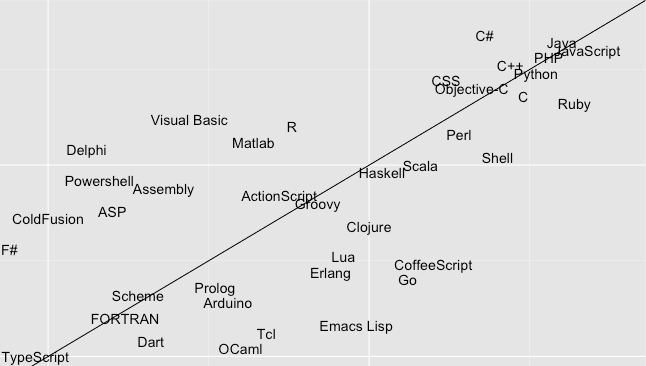
\includegraphics[width=1.0\textwidth]{lang-rank-114-wm.png}
\end{figure}

The advantages of transpilers often mean that less can be written in order to achieve the same functionality in its targeted language. Simple common activities such as array iteration, class extension, and appending vendor prefixes can become unnecessarily ceremonious especially in the case of JavaScript when shimming non-existent functionality. These transpilers can offer an alternative means in which to achieve the same results with less code and effort required on the part of the developer.

Google's Dart ``is a new platform for scalable web app engineering'' which comes in the form of several tools. First there is Dart the language which is an alternative to writing plain JavaScript with a host of additional built-in and libraries language features akin to Java \cite{Fortuna}. Second there is DartVM a virtual machine that comes as a standalone program and also happens to be embedded in the Google Chrome browser. The DartVM works similarly to a typical JavaScript virtual machine with the difference being it interprets \texttt{.dart} code instead of \texttt{.js} with significant performance advantages \cite{Schneider}. Lastly there is the dart2js compiler, which is effectively a backwards compatibility tool to ensure any application created on the Dart platform will still work through conventional means.

Microsoft's TypeScript by its own admission ``is a typed superset of JavaScript that compiles to plain JavaScript.'' which makes it very flexible alternative. This effectively means that you can continue to write plain JavaScript and no restrictions will be imposed by the TypeScript transpiler. This helps greatly if a developer already has a large JavaScript codebase which they wants to utilise during the development of a large scale application. TypeScript offers some of the inherently missing language features of JavaScript such as type annotations, classes, interfaces and modules. There are also plans to support ECMAScript 6 features once it becomes the standard. Another positive remark about the output produced by the TypeScript transpiler is it produces rather legible JavaScript making it easy to see the relationships between the source and target languages.

Because the compile target of these transpilers is JavaScript it is possible to take advantage of them when developing mobile web applications such as video games. When project development first started, TypeScript was the target language because it was syntaxitcally similar to that of ActionScript 3, where my background lies. However, due to the immaturity of the project at the time and a lack of core JavaScript knowledge on my part, it was later ditched as time constraints prevented the investment of fully learning its quirks. Also it felt like working at this level of abstraction could potentially lead to delays when debugging later in development. However, as of \textit{April 2014} close to the time of writing, the specification for TypeScript 1.0\footnotemark has been finalised and its current status is \textit{stable}. Going forward after this project I am eager to re-evaluate it now that it has had time to mature.

\footnotetext{\url{http://www.typescriptlang.org/Content/TypeScript\%20Language\%20Specification.pdf}}

JavaScript is typically created as separate \texttt{.js} text files that are then referenced in a \texttt{.html} document by \texttt{<script>} tags. When the web browser finds scripts linked by these tags it will request them from the web server and inject them into the document once loaded. This presents a few problems for large and complex web applications which will often require many scripts each having to be requested and loaded synchronously. Every one of these request has an overhead, which is compounded when a vast quantity are being made. This can lead to suboptimal load times.

To combat this problem a developer could attempt to write all their code in one \texttt{.js} file. This file can quickly become colossal making it difficult to manage and refactor, especially on large scale projects. Alternatively the developer can split their code into several \texttt{.js} files that will all have to be referenced by a corresponding \texttt{<script>} tag. Therefore the more organised the codebase becomes the more requests the browser has to make. The developer also has to micromanage these \texttt{<script>} tags to ensure their ordering is correct. The ordering is important because one script could be referencing another that has not yet been loaded, thus causing runtime errors. This approach also presents issues when attempting to introduce software engineering best practices such as unit testing because the interdependencies between these scripts are not clearly defined.

One solution to this common problem is the \textit{module} design pattern. JavaScript has an official name ECMAScript, and version 5.1 (ECMA-262\footnotemark) is the current standard. However, this present language specification does not support modules. The 6th version\footnotemark of the ECMAScript specification is currently being drafted with plans to include modules but until then developers must seek other alternatives.

\footnotetext{\url{http://www.ecma-international.org/ecma-262/5.1/}}
\footnotetext{\url{https://people.mozilla.org/~jorendorff/es6-draft.html}}

There are a variety of libraries that offer solutions such as RequireJS\footnotemark, HeadJS\footnotemark and yepnope.js\footnotemark. After testing and evaluating these libraries Browserify\footnotemark presented itself as the simplest and the most supported amongst the Node.js community. Browserify enables developers to write their JavaScript code in numerous files and when one file requires another it can be injected via the \texttt{require(`example');} function. Once a developer has written all their code they can recursively bundle all their modules starting with a root module similar to that of a main class in conventional programming languages. This provides the developer with the best of both scenarios as all their code will be built into a single \texttt{.js} file (including their external libraries), while allowing for easy management and refactoring of their core codebase through individual source files.

\footnotetext{\url{http://requirejs.org/}}
\footnotetext{\url{http://headjs.com/}}
\footnotetext{\url{http://yepnopejs.com/}}
\footnotetext{\url{http://browserify.org/}}

Most might think that this will in turn cause complications when debugging. As when the code breaks it will do so in the colossal \texttt{.js} file that the browser is running. This is where source maps come in. Source maps provide linkage between the original \texttt{.js} source files and their bundled counterparts making breakpoints and stepping through code painless. \cite{Seddon}

This process can also be made seamless by Watchify which automatically recompiles the Browserify bundle whenever a module file has been updated. This allows for the developer to work on their original source files and as soon as the file has been saved it have rebuilt the bundle ready to reloaded in the browser for testing.

After the modules have been bundled a further step called minification which involves taking legible JavaScript and compressing it down into its most minimal form by removing unnecessary characters such as a whitespace and shrinking instance names. This process can further decrease the \texttt{.js} file size making load times marginally faster while also partially obfuscating the original code from prying eyes.

\cite{Hanselman} proclaimed that JavaScript has become akin to a assembly language for the web. Which is the impression a lot of people will get when taking a peek at the source of popular website such as Googlex or Facebook. This is some what understandable given the that JavaScript is as low-level as developers can get when programming for the web. However, a happy side effect of being closely tide with the web is it has become now one of the most portable languages to date, because every web enabled device has a browser, and every browser has a JavaScript virtual machine. This makes JavaScript a very cross-platform language to develop games with and reaching a wide audience is key when maximising chances for success.

To keep my project structure and programming semantics organised the MVC (model view controller) design pattern was to be employed in development. However, because of the inherent structure of web applications a controller often is not a ``true'' controller and mislabelled which has led to the term MV* framework implying a substitution of the controller with a more appropriate alternative. Development began initially using TypeScript and then later moving to plain JavaScript, inexperience with the language rapidly led to jumbled spaghetti code. A MV* frameworks looked like an appealing solution that would assist with retaining a legible codebase.  Which became imperative when frequently switching between other coursework projects that also required prolonged development in differing programming languages.

As with most JavaScript frameworks there are countless variants on offer which made it daunting to select one. It was important to make a firm decision as limiting time constraints prevented me from investing time in learning the pros and cons of each. TodoMVC\footnotemark is a project with the intent of assisting developers select a JavaScript MV* framework. TodoMVC provides developers with a simple todo web application constructed with each of these varying MV* frameworks, allowing them to quickly browser the source code of each and determine whether it suits their needs.

\footnotetext{\url{http://todomvc.com/}}

Backbone.js\footnotemark was chosen because of its flexibility, large community following, and modular design. As described in a presentation given by \citet{Bull} Backbone.js is the equivalent of a \textit{knife/spoon/fork} on a camping trip. This analogy represents its modularity implying that there is no imposed exclusivity between its internal components. This allowed me to gradually implement the use of its Model, View, Collection, and Router classes throughout my development process not forcing me to learn everything at once but only when it was required.

\footnotetext{\url{http://backbonejs.org/}}

During this project development a slue of various tools and applications were evaluated for use features and work flow efficiency. The most fundamental tool required is that of a text editors and/or IDE (integrated development environment). They help to maximise the output of a developer by offering efficient procedures such as autocompletion, refactoring and build automation.

Brackets\footnotemark[27] is an open source code editor for web designers and front-end developers constructed with HTML, CSS and JS and maintained by Adobe. It has a comprehensive suite of plugins\footnotemark[28] providing developers a great way to customise it to suit their needs. As the project is open source it allows developers to create and submit their own plugins if their niche has yet to be filled. One of the most useful features is the live preview mode letting me type code while viewing its results instantaneously in the browser. Tweaking the aesthetics of \textit{MindFlip} was easy, changes to colours and styles declaration were instantly visible through live preview which made decisions as to whether they were appropriate swift. The nested nature of this editor being built with the languages it is providing the means to edit also benefits from the inherent portability of these languages making it avaliable cross platform on Windows, Linux and OSX.

\footnotetext{\url{http://brackets.io/}}
\footnotetext{\url{https://brackets-registry.aboutweb.com/}}

Sublime Text is a sophisticated text editor for code, markup and prose \footnotemark. A popular editor amongst the developer community with is broad coverage of languages and clever short-cuts. The editor is very veritable and can be customised down to the minutiae with packages and plugins many of which can be found on Package Control\footnotemark. It has a very DIY approach expecting users to setup their own build commands and identify the packages that are applicable to their workflow. This has a large learning curve which can discourage some developers that work from a high level of abstraction. Nevertheless, developers looking for such fine control over their development experience will be pleased with the variety of configurations options on offer. Sublime Text is free for evaluation with no time constraints and with the only difference from the full version being a faint \textit{``UNREGISTERED''} water mark.

\footnotetext{\url{http://www.sublimetext.com/}}
\footnotetext{\url{https://sublime.wbond.net/}}

JetBrains WebStorm is a comprehensive IDE for web development. It has support for many of the preprocessor languages talked about in section \ref{sec:transpilers} right out of the box without plugins and add-ons having to be seeked out by the developer. This was used for the initial stretch of development and boosted the project's productivity by not having to spend lengthy periods of time ironing out the details of the development stack should function. Later in development this IDE was ditched in favour of Adobe Brackets because of performance and incompatibilities with the desired development stack.

One of the challenges that faces mobile developers is how to package their applications for the mobile platform, which spans such a wide variety of hardware and operating systems (iOS\footnotemark, Android\footnotemark, Windows Phone\footnotemark, Ubuntu\footnotemark). This poses a problem especially for the smaller companies as to develop native variants of an application for each platform while retaining a common vision is demanding on both financial and chronological frontiers. Larger companies that facilitate and accommodate such resources, can however frequently benefit from more seamless experience. Most native applications built with their corresponding software development kits (SDKs) which have direct access to device specific application programming intefaces (APIs). This often results in native applications having faster performance and better system user interface integration. Native applications compile to binary machine code that is then interpreted via its relative hardware architecture making it vastly faster than JavaScript which is interpreted at run-time via a browser or web-view. This is most apparent when it comes to developing 3D gaming experiences as these can often be most the most performance taxing, \cite{Kulloli}.

\footnotetext{\url{http://www.apple.com/ios/}}
\footnotetext{\url{http://www.android.com/}}
\footnotetext{\url{http://www.windowsphone.com/}}
\footnotetext{\url{http://www.ubuntu.com/phone}}

When comparing HTML5 based mobile applications to native there was another significant disadvantage as there was no way to access device APIs. Such APIs are required to make use of the most hardware features on mobile devices such as the camera, device orientation and battery status. Especially considering that each API varies dependant on operating system and then again on hardware specification. For instance not all mobiles have front facing cameras or high-dpi (dots per inch) screens but a vast majority do. So it becomes quite a challenge when trying to build an application that adapts from phone-to-phone without excluding a particular sector of an audience from the core user experience, \cite{Charland}.

A project with the sole purpose of remedying such issues is that of PhoneGap a mobile development framework originally created by a company called Nitboi. After PhoneGap began to make strides the company was purchased and enveloped by Adobe in 2011, \cite{Adobe}. Then after the project matured under Adobe's supervision the project was donated to the Apache Software Foundation. This was to ensure that the project was properly maintained when made open source under the Apache License Version 2.0\footnotemark. A formality due to this hand over was that the open source variety of the project had to operate under a different name to avoid trademark ambiguity, \cite{Leroux}. Adobe's PhoneGap still functions as a separate entity as a distribution of Apache Cordova offering services such as cloud compilation\footnotemark.

\footnotetext{\url{http://www.apache.org/licenses/LICENSE-2.0.html}}
\footnotetext{\url{https://build.phonegap.com/}}

Apache Cordova\footnotemark is a platform for building native mobile applications using HTML, CSS and JavaScript. It achieves this by providing developers with a set of relative device APIs that allow for access of functions previous obfuscated from web technologies by the native system. It also assists with handling a lot of the cross-platform concerns previously mention when targeting multiple platforms and device hardware.

\footnotetext[35]{\url{http://cordova.apache.org/}}

CocoonJS is a comprehensive HTML5 app and game development platform created and developed by Ludei. During the course of this project the platform was functional but still improving some of its vital features. Earlier this year in version \texttt{1.4.7} they introduced \footnotemark GPU accelerated WebGL across a widespead of mobile platforms. This feature was innovative at the time because until then because no equivalent existed. Since earlier this year they have made huge strides in improving their platform as well as partnering with similar companies and developers. The disadvantages of CocoonJS at the moment are its compilation service is closed source and although it is currently free Ludei have made no commitments to keeping it that.

\footnotetext{\url{http://blog.ludei.com/cocoonjs-1-4-7/}}

It took me awhile to finally settle upon the debugging solution of my development stack and I tried a few approaches with varying success. It was important to be able to quickly prototype on my desktop computer as well as my mobile devices. On desktop computers this is relatively easy as most desktop browsers applications have built in development tools with a variety of features. However, understandable this is not the case commonly on mobile browsers as screen space is limited and it would be difficult to convey the vast streams of data are under the hood of a typical web application. Even the bare minimum tools such as a console are often absent in mobile browsers which are a necessity when trying to diagnose runtime errors in generated by JavaScript as well as reading the output \texttt{console.log()}.

Apache Ripple\footnotemark is a companion project of Cordova consists of a web based mobile environment simulator design to emulate the conditions of a packaged Cordova application. It has options for manipulating mobile specific features such as GPS (global positioning system) geolocation and device orientation. This can be useful for developers when rapidly prototyping an application that makes use such mobile specific features. This solution was used for a while until the lack of up-to-date documentation and dwindling support hampered progress during early development.

\footnotetext[36]{\url{http://ripple.incubator.apache.org/}}

Weinre\footnotemark (web inspector remote) is a debugger application created by Patrick Mueller\footnotemark who is also a contributor to the Apache Cordova project. This application works similar to the built-in desktop browser debuggers and inspectors with the added bonus of having a remote target. By including a remote JavaScript file hosted on a local weinre server the mobile device can be linked letting it send and receive debugger data from the server. This lets developers inspect and manipulate the mobile devices web browser. The key issue that prevented the further use of this application in the project's development was that in combination with Apache Cordova it was not able to log any information before the script was loaded and the console was initialized. So when it came to analysing the initial portion of an application's lifecycle the data generated was restricted by this dependency.

\footnotetext{\url{http://people.apache.org/~pmuellr/weinre/docs/latest/Home.html}}
\footnotetext{\url{http://muellerware.org/}}

Adobe Edge Inspect\footnotemark previously known as Adobe Shadow is a tool built on top of Weinre that lets developers preview and inspect across multiple devices concurrently. 
When it was being assessed for use in this project's development the free version was limited to testing on one device, since then it has become exclusively a paid product. Another disadvantage that came with using this solution is the web application had to be viewed through their Adobe Edge mobile application similar to that of a browser. This made it impossible to debug the game through its targeted environment bundled within a Cordova application.

\footnotetext[39]{\url{http://html.adobe.com/edge/inspect/}}

Chrome DevTools\footnotemark was definitely the most comprehensive and painless solution discovered during development. DevTools encapsulates mobile emulation\footnotemark as well as remote debugging\footnotemark of Android's WebView on versions 4.0 and above which Cordova uses to display the embedded web content. During development some of these features were classified as ``experimental'' but still accessible through Chrome Canary\footnotemark, a custom variant of Google's browser designed for developers and early adopters of fringe web technologies. DevTools provided a quick and effective way to iteratively test the game first on the desktop platform, a mobile emulation, and finally when deployed on mobile devices.

\footnotetext{\url{https://developers.google.com/chrome-developer-tools/}}
\footnotetext{\url{https://developers.google.com/chrome-developer-tools/docs/mobile-emulation}}
\footnotetext{\url{https://developers.google.com/chrome-developer-tools/docs/remote-debugging}}
\footnotetext{\url{https://www.google.co.uk/intl/en/chrome/browser/canary.html}}

The key issue HTML5 is tackling on the mobile platform is portability. OEMs will continue to improve and innovate their product lines at different rates relative to what is profitable and marketable. As the cost of the technology required to construct these devices plummets so does the cost to improve and innovate. The technology life-cycle of mobile devices is short in contrast to that of web specifications. If developers desire cross platform compatibility there are many moving targets they have to hit when it comes to native development; hardware specifications, operating systems, store requirements, and official software development kits. Hitting these targets in an ever fluctuating landscape demands much of a developer's focus, which could be better spent more effectively improving a game's overall quality and design. The web has proved itself as a stable and universal platform on desktop computers and eventually this will be implemented fully on mobile devices.

Currently the platform on mobiles is lacking full support of accelerated canvas and WebGL in stock mobile browsers. However, this does not have to discourage developers as the support is on its way. In the mean time developers can use hybrid mobile application frameworks such as Apache Cordova and CocoonJS to get a head start on utilising edge features. Once native support for these features is introduced their original source code will be instantaneously be compatible not even requiring compilation. As processing power on mobile devices increases other concerns such as performance will eventually become irrelevant and then a developers focus will skew towards the architecture and accessibility of their code rather its over engineered optimisation.

The future of JavaScript looks bright according to the creator \citet{Eich}. ECMAScript 7 intends to introduce language features such as overloadable operators, observers, value objects, and SIMD (single instruction, multiple data) intrinsics. The use of SIMD and low-level value objects in JavaScript will lead to near native performance while being widely compatible across processor architectures such as Intel's SSE, AMD's AVX, and ARM's NEON popularly used in mobile devices. He goes on to promote his extensible web manifesto\footnotemark that notably focuses on adding safe and secure low-level capabilities to the web platform as well as simplifying and streamlining the standardisation process by tightening the feedback loop between committees and developers.

\footnotetext{\url{http://extensiblewebmanifesto.org/}}

The video games industry will continue to grow in scope. Consoles such as the \textit{Nintendo Wii} have had widespread success across demographics in recent years. Victories such as these are bringing this creative medium to mainstream society. I feel mobile devices will similarly perpetuate the medium as they become common place in our daily lives. With the web growing alongside these devices it is a natural progression that they become intertwined. This is already happening in projects such as Ubuntu for Phones and Firefox OS. The web platform presents attractive prospects for game developers offering lasting portability which as performance issues become less of a problem will become their dominant priority. This project overall has been successful and has encouraged me to seek out and research this platform thoroughly. I feel my newly acquired skills and experience will hugely useful going forward with my career in industry.

\clearpage
\bibliography{5939968}

\end{document}

